\secnumberlesssection{ANEXOS}

\begin{itemize}
    \item Anexo 1: Diagrama explicativo del sistema de Óptica Activa.
        \\
        \vspace{3.5cm}
        \includegraphics[width=12cm]{figures/diagram_oa} \\
        \vspace{3.5cm}


    \item Anexo 2: Extracto de un registro de log del UT 1.
        \begin{myverbatim}[caption={Plantillas TTP},label={myverbatim:ttp}]
        Sep 22 00:25:24 wt1tcs logManager[318044]: wt1tcs  00:25:23>-START DET EXP / Start exposure [lt1iab]
        Sep 22 00:25:24 wt1tcs logManager[318044]: wt1tcs  00:25:23> TEL M2 DECOFF = 0.0079 / [arcsec] DEC correction offloaded by M2 to axis by AG [lt1m2]
        Sep 22 00:25:24 wt1tcs logManager[318044]: wt1tcs  00:25:23> TEL M2 RAOFF = 0.0013 / [arcsec] RA correction offloaded by M2 to axis by AG [lt1m2]
        Sep 22 00:25:24 wt1tcs logManager[318044]: wt1tcs  00:25:23>-START DET CHIP WIPE / CCD start wipe action [lt1iab]
        Sep 22 00:25:24 wt1tcs logManager[318044]: wt1tcs  00:25:23> DET EXP NO = 821 / Unique exposure ID number [lt1iab]
        Sep 22 00:25:24 wt1tcs logManager[318044]: wt1tcs  00:25:23>-START DET CHIP WIPE / CCD start wipe action [lt1iab]
        Sep 22 00:25:24 wt1tcs logManager[318044]: wt1tcs  00:25:23> DET WIN1 UIT1 = 0.300000 / user defined subintegration time [lt1iab]
        Sep 22 00:25:24 wt1tcs logManager[318044]: wt1tcs  00:25:23> DET EXP WIPETIM = 0 / wipe before starting exposure in a loop [lt1iab]
        Sep 22 00:25:24 wt1tcs logManager[318044]: wt1tcs  00:25:23> DET OUT1 GAININD = 4 / Gain index for output [lt1iab]
    
        \end{myverbatim}

    \item Anexo 3: Diagrama de flujo del proceso de solución.
        \\
        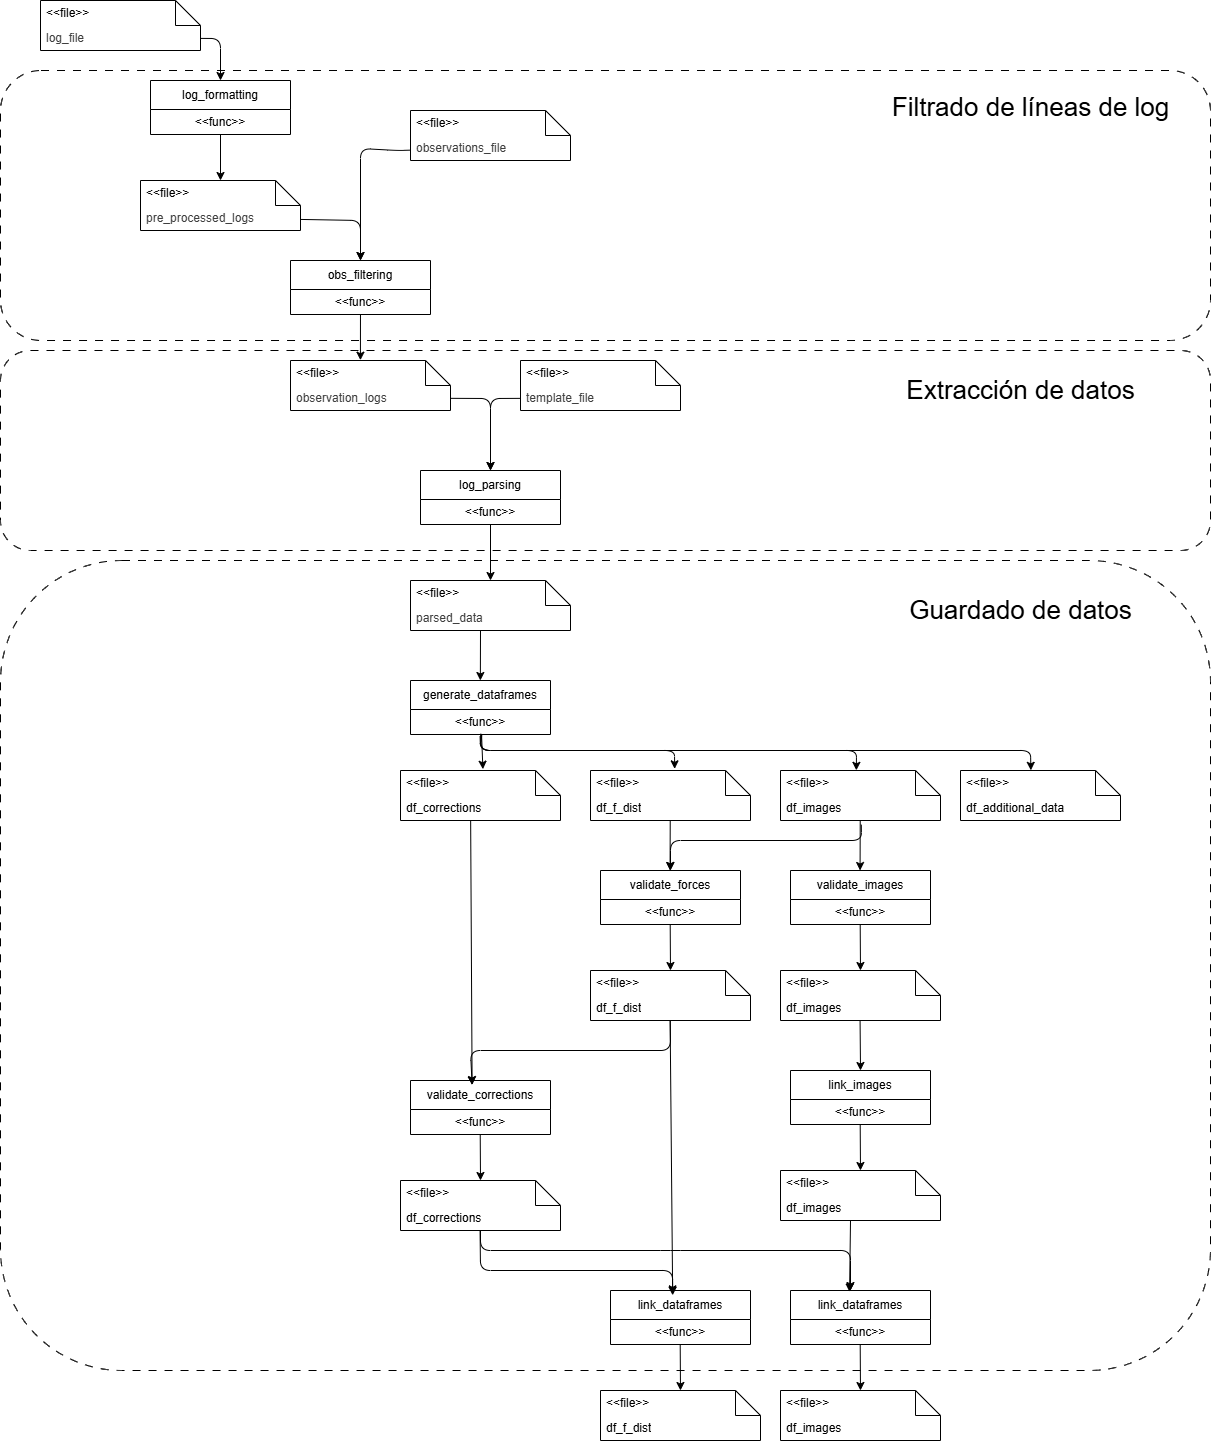
\includegraphics[width=11cm,height=14cm]{figures/flow_diagram.png} \\

\end{itemize}


\begin{itemize}
    \item Diccionario 1: Frente de Onda

    El frente de onda es una superficie imaginaria que representa los puntos correspondientes de una onda que vibra al unisono. Cuando ondas idénticas con un origen en común viajan a través de un medio homogéneo, los senos y picos correspondientes a cada uno se mantienen en fase \cite{britannica2022front}. 

    \item Diccionario 2: Sensor de frente de onda

    Es un sensor diseñado para calcular las aberraciones de una imágen mientras se toma la misma. Generalmente las aberraciones son producidas por ladeos en los frentes de onda, presentes en imágenes que capturan objetos al otro lado de la atmósfera \cite{platt2001sh}

     \item Diccionario 3: Librería Template Text Parser

     Template Text Parser, o TTP, es una librería de Python que permite la extracción de datos de texto semi estructurado usando plantillas, manteniendo un rendimiento relativamente rápido. Iniclamente fue desarrollado para permitir el acceso procedural a datos producidos por las consolas de aparatos de red, sin embargo, actualmente puede ser usada para extraer cualquier texto semi estructurado que contenga patrones de repetición distintivos \cite{dmulyalin2021ttp}.
\end{itemize}